\documentclass{beamer}
\usepackage{mathtools}
\DeclarePairedDelimiter{\ceil}{\lceil}{\rceil}
\usepackage{algorithm}
\usepackage{algpseudocode}
\usepackage[english]{babel}
\usepackage[utf8]{inputenc}
\usetheme{Madrid}
\usecolortheme{dolphin}

\logo{\includegraphics[width=0.1\textwidth]{sdu_segl}}

\title{Interaktion og interaktionsdesign}
\author{Steven Gøhler}
\begin{document}
\begin{frame}
\titlepage
Redegør for principper og problematikker vedrørende det visuelle design af et grafisk interface.
\end{frame}

\begin{frame}
  \frametitle{Overview}
  \tableofcontents
\end{frame}

\section{Interface}
\begin{frame}
\frametitle{Interface}
  \begin{columns}[T]
    \begin{column}{.5\textwidth}
	  \begin{itemize}
		\item Interaktion mellem bruger og system
		\item Skeuomorphism/Flat design
	    \item Vælge med omhu
	  \end{itemize}
    \end{column}
    \begin{column}{.5\textwidth}
      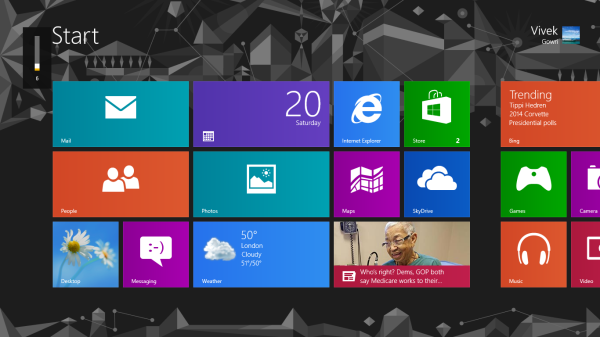
\includegraphics[width=\textwidth]{interface.png}
    \end{column}
  \end{columns}
\end{frame}


\section{Skeuomophism}
\begin{frame}
\frametitle{Skeuomophism}
  \begin{columns}[T]
    \begin{column}{.5\textwidth}
	  \begin{itemize}
		\item Hold det simpelt
		\item Ram visuelle ting brugeren allerede kender
		\item Baseret på genkendelse
	  \end{itemize}
    \end{column}
    \begin{column}{.5\textwidth}
      
\includegraphics[width=\textwidth]{button.jpg}
    \end{column}
  \end{columns}
\end{frame}

\section{Flat-design}
\begin{frame}
  \frametitle{Flat-design}
  \begin{columns}[T]
    \begin{column}{0.5\textwidth}
      \begin{itemize}
	    \item Føles pænt og rart at se på
	    \item Let læseligt
	    \item Bruger tit gruppering
	    \item Godt til kort og navigering
      \end{itemize}  
    \end{column}
    \begin{column}{.5\textwidth}
      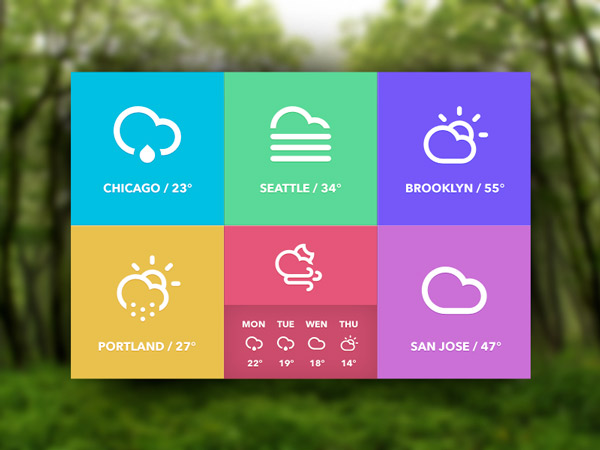
\includegraphics[width=\textwidth]{flat.jpg}
    \end{column}
  \end{columns}
\end{frame}


\section{Gestalt's regler}
\begin{frame}
\frametitle{Gestalt}
  \begin{columns}[T]
    \begin{column}{.5\textwidth}
	  \begin{itemize}\setlength{\itemsep}{30pt}
		\item Figur/Grund (Figure/groud)
		\item Ensartethed (Similarity)
		\item Nærhed (Proximity)
	  \end{itemize}
    \end{column}
    \begin{column}{.5\textwidth}
      \includegraphics[scale=0.25]{figure.pdf}\\
      \includegraphics[scale=0.2]{sim.pdf}\\
      \includegraphics[scale=0.16]{proximity.pdf}
    \end{column}
  \end{columns}
\end{frame}


\section*{Gestalt's regler}
\begin{frame}
\frametitle{Gestalt}
  \begin{columns}[T]
    \begin{column}{.5\textwidth}
	  \begin{itemize}\setlength{\itemsep}{35pt}
		\item Videreførelse (Continuation)
		\item Afslutning (Closure)
		\item Fælles skæbne (Common fate)
	  \end{itemize}
    \end{column}
    \begin{column}{.5\textwidth}
      \includegraphics[scale=0.3]{continuation.pdf}\\
      \includegraphics[scale=0.2]{closure.pdf}\\
      \includegraphics[scale=1]{CommonFate.pdf}
    \end{column}
  \end{columns}
\end{frame}


\end{document}